% Beamer slide template prepared by Tom Clark <tom.clark@op.ac.nz>
% Otago Polytechnic
% Dec 2012

\documentclass[10pt]{beamer}
\usetheme{CambridgeUS}
\usepackage{graphicx}
\usepackage{fancyvrb}
\usepackage{ulem}
\newcommand\codeHighlight[1]{\textcolor[rgb]{1,0,0}{\textbf{#1}}}

\title{Bacula Architecture and Configuration Files}
\author[IN719]{Systems Administration}
\institute[Otago Polytechnic]{
  Otago Polytechnic \\
  Dunedin, New Zealand \\
}
\date{}

\begin{document}

%----------- titlepage ----------------------------------------------%
\begin{frame}[plain]
  \titlepage
\end{frame}

%----------- slide --------------------------------------------------%
\begin{frame}
  \frametitle{Bacula Architecture}
 
\begin{figure}
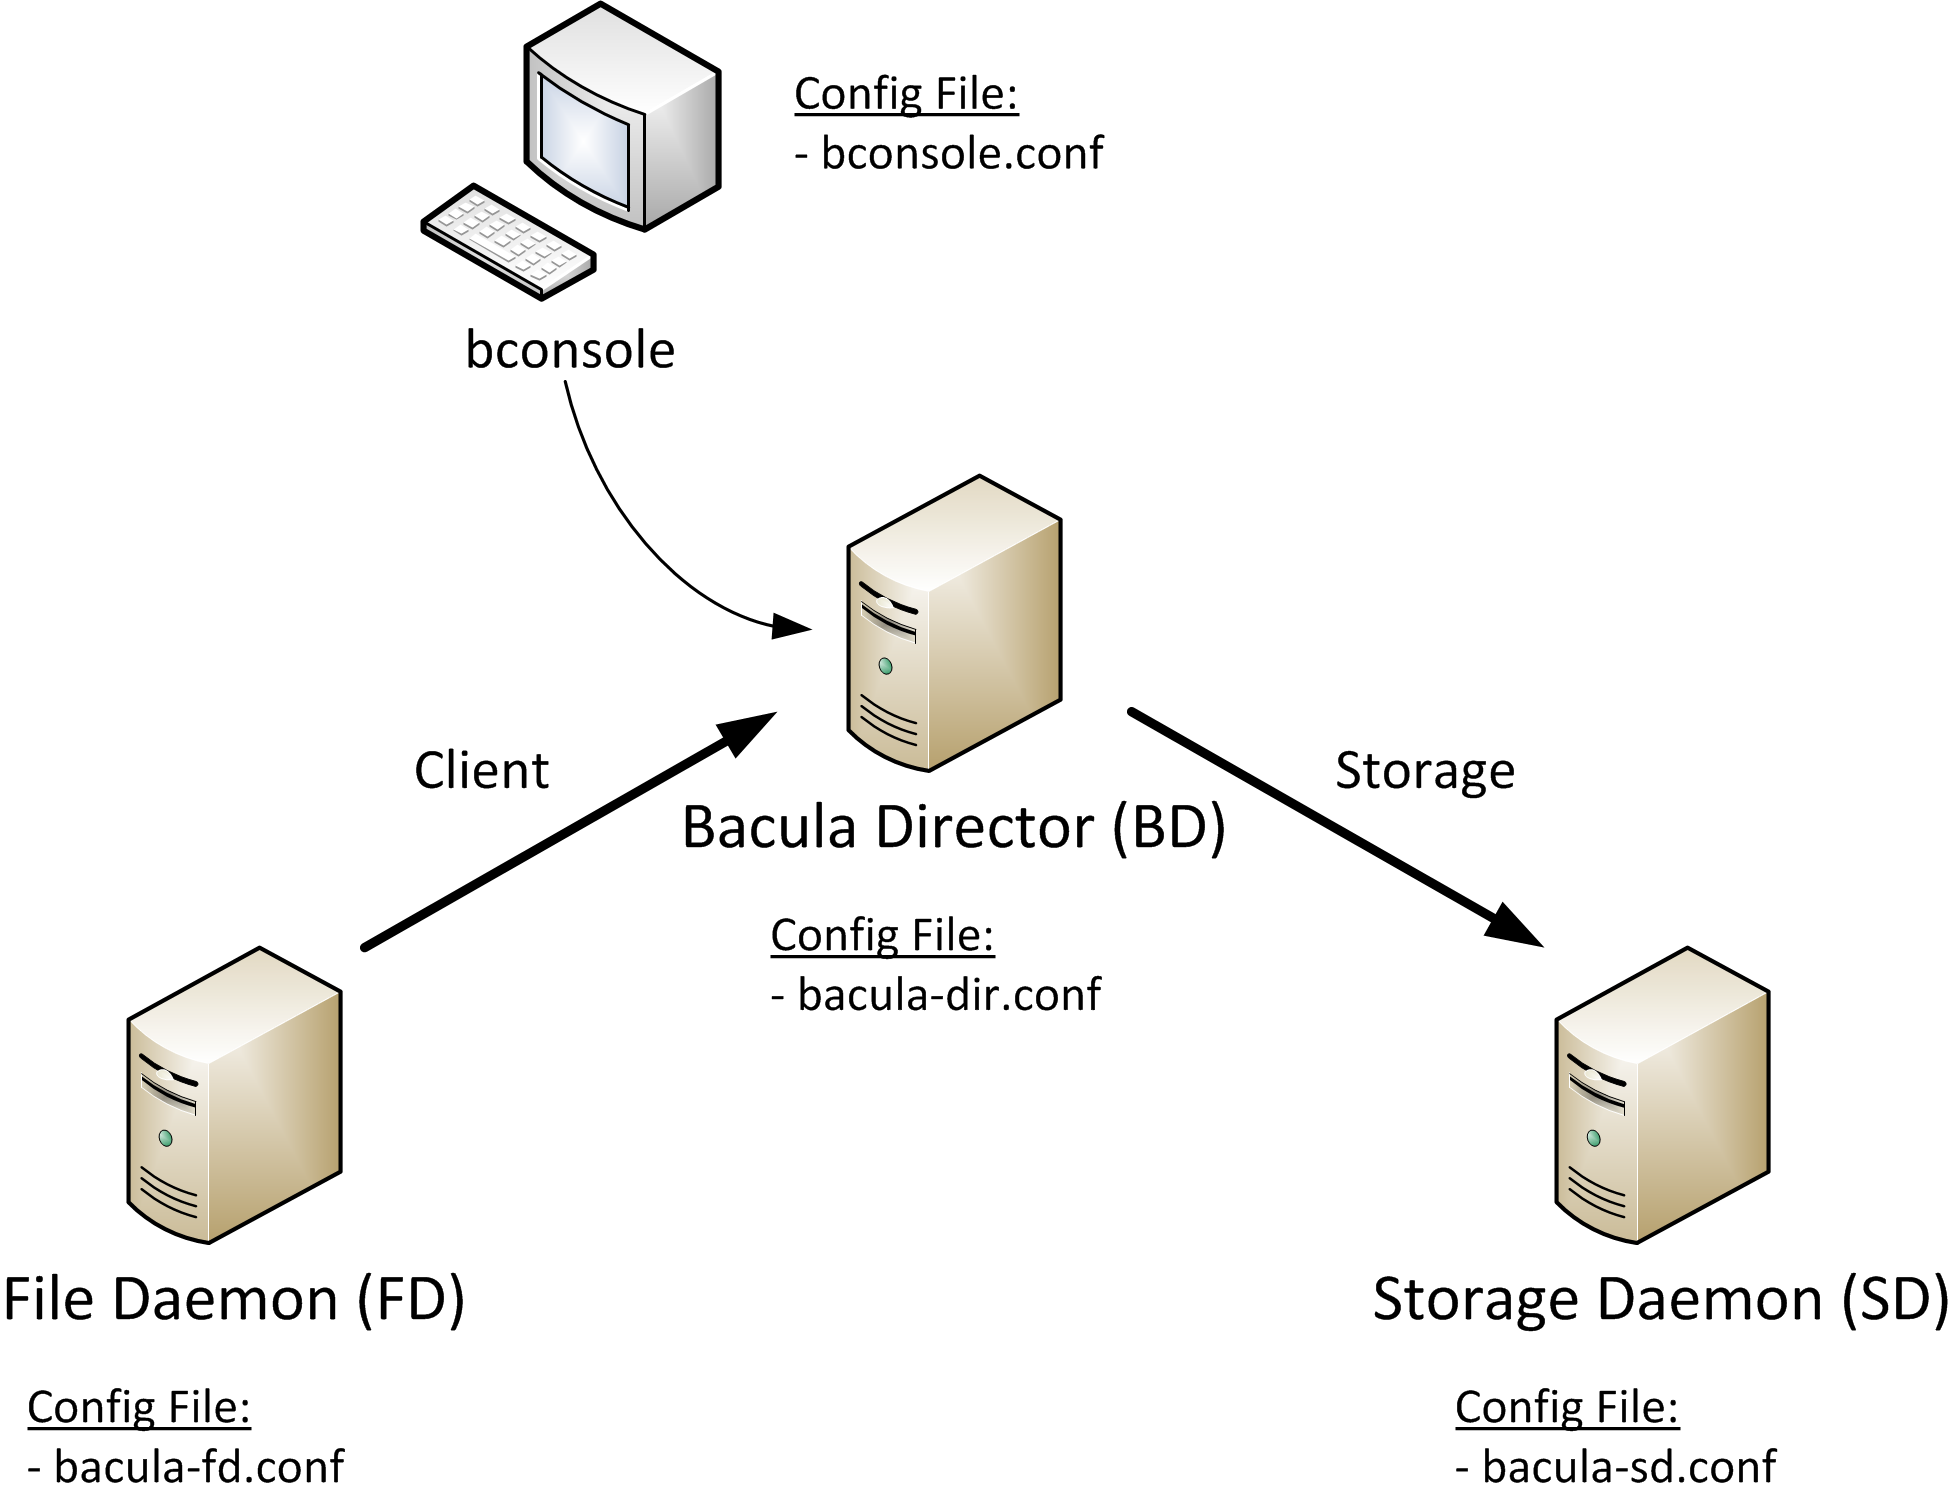
\includegraphics[width=9.5cm]{./figures/BaculaSchema.png}
\end{figure}

\end{frame}

%----------- slide --------------------------------------------------%
\begin{frame}
  \frametitle{Bacula Objects}

\begin{figure}
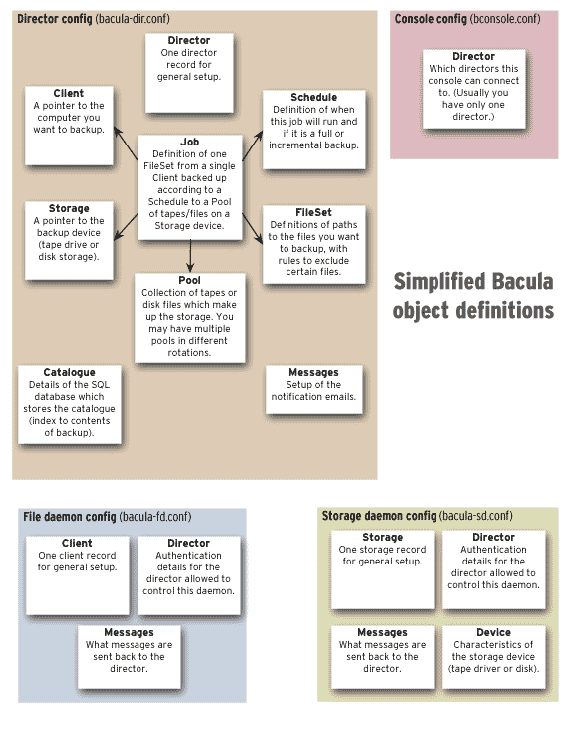
\includegraphics[width=5.8cm]{./figures/bacula-objects.png}
\end{figure}

\vspace{-0.5cm}
{\scriptsize Source:  \url{http://www.bacula.org/5.2.x-manuals/en/main/main/Customizing_Configuration_F.html}}

\end{frame}

%----------- slide --------------------------------------------------%
\begin{frame}
	\frametitle{Network Authentication}

\begin{figure}
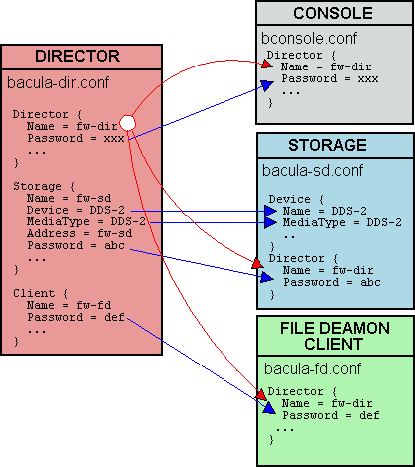
\includegraphics[width=5.8cm]{./figures/BaculaAuth.png}
\end{figure}

%\vspace{-0.5cm}
{\scriptsize Source:  \url{http://www.bacula.org/5.2.x-manuals/en/main/main/Customizing_Configuration_F.html}}	
	
\end{frame}

%----------- slide --------------------------------------------------%
\begin{frame}
  \frametitle{Resources}
 

\begin{itemize}


\item Tutorial-style reference (based on older version):\\ \url{http://wiki.defcon.no/guides/bacup/bacula}
\item `Official' Tutorial from Documentation:\\ \url{http://www.bacula.org/5.2.x-manuals/en/main/main/Brief_Tutorial.html}
\item Documentation:\\ \url{http://www.bacula.org/5.2.x-manuals/en/main/main/Bacula_Main_Reference.html}
\item Cheat sheet:\\ \url{https://workaround.org/bacula-cheatsheet/}

\end{itemize}
\end{frame}


\end{document}
